\section{The application}
\label{sec:website}

The interface is one page (Figure~\ref{fig:dashboard}). A \emph{Now} panel shows the current sleepiness on the KSS scale and the cognitive load on the TLX scale, each with a 90\% interval and its verbal anchor, a sentence giving the predicted time of reaching KSS~7, and the breakdown of the estimate into the rhythm model, time on task, check-ins, reaction tests and the webcam. An \emph{Eyes and head} panel shows the live video with the eye landmarks drawn over it and traces of eye closure and head pitch for the last 30~s; the alarms of Section~\ref{sec:system} appear here. A timeline shows the rhythm model, the twin's estimate with its 90\% band, check-ins, reaction tests, the minutes covered by the webcam and the forecast for the next 8~hours, with a second panel for workload. What-if buttons overlay the forecast under a 15-minute break, a bedtime of 23:00, or continuing without a break. Further panels let the person mark what they are doing and when they woke, show what the twin has learned about them, and export or delete their data. The check-in dialog presents the KSS with its original anchors and the six NASA-TLX subscales, and the reaction test runs full screen.

For transparency, each main panel has a ``How is this predicted?'' explanation that states the model behind the number, its sources and its limits, with the evaluation results reported in this paper. The same text is kept in the repository as \texttt{docs/SCIENCE.md}.

A demo mode loads one simulated day so that the interface can be explored without a camera; it is marked as demo data and kept apart from the person's own records. Figure~\ref{fig:dashboard} uses demo data.

\begin{figure}[p]
  \centering
  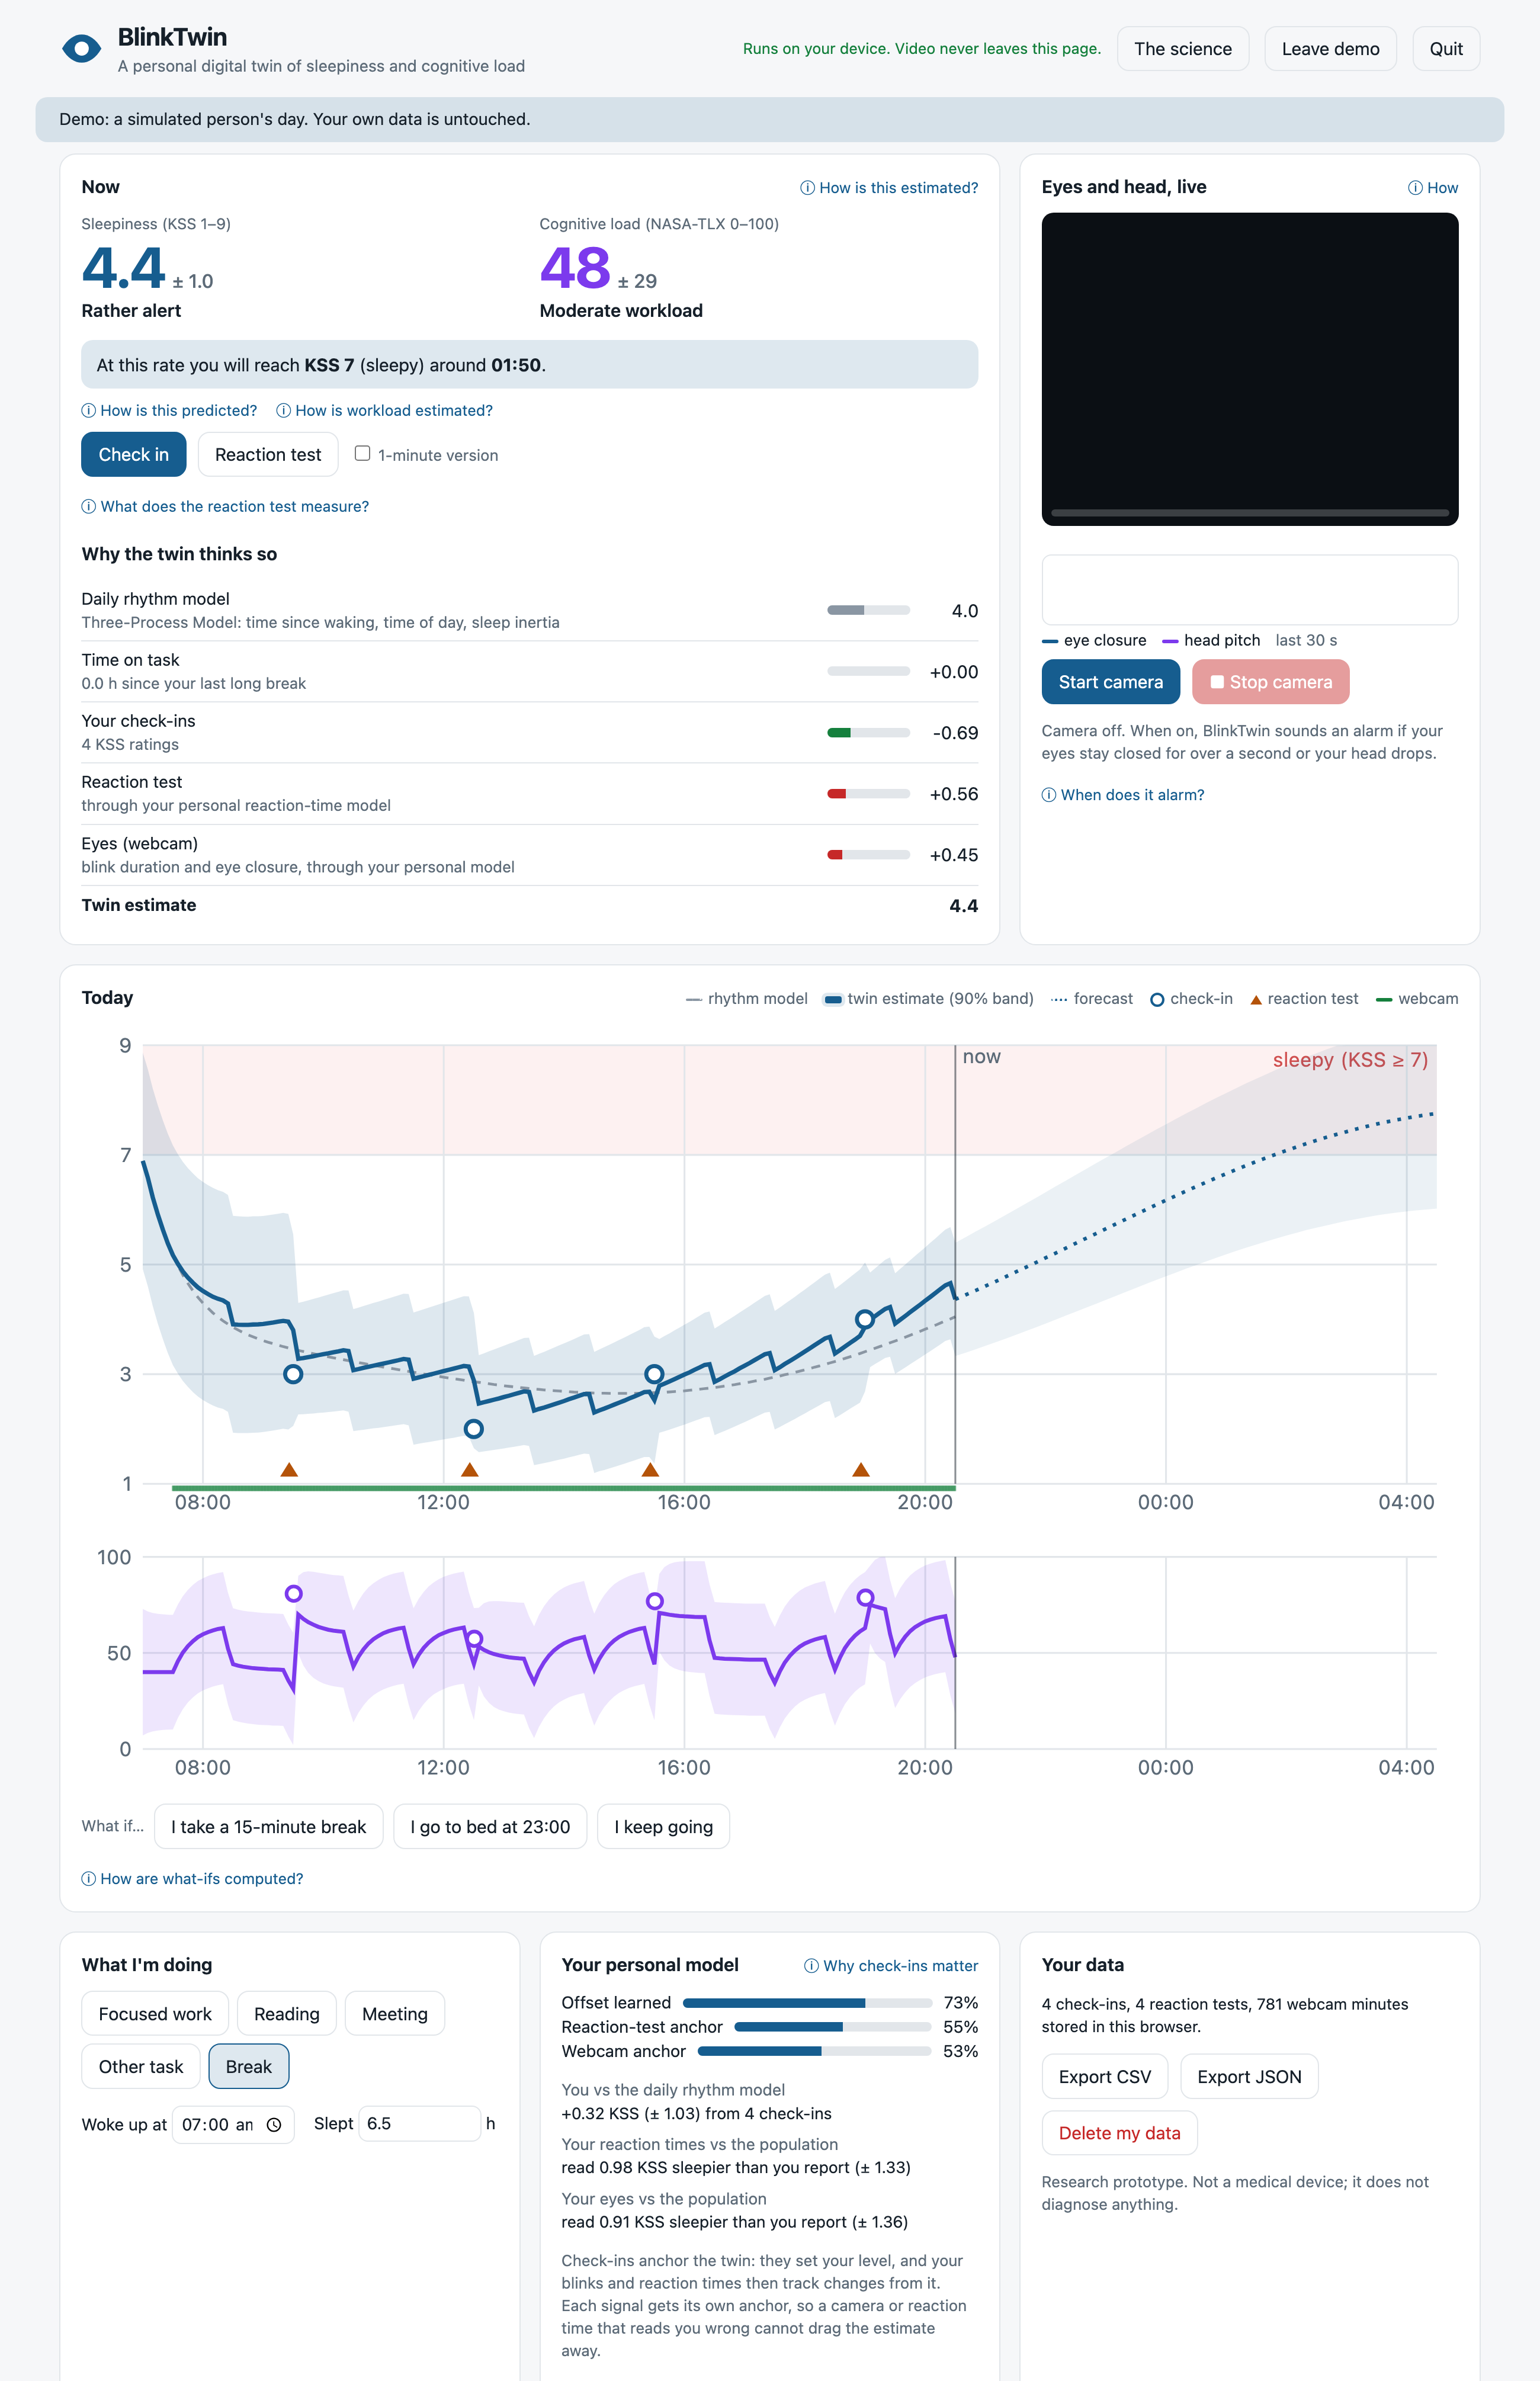
\includegraphics[height=0.88\textheight]{../docs/img/dashboard.png}
  \caption{The BlinkTwin dashboard during a demo day (simulated data, camera off). Top: current state with 90\% intervals and the breakdown of the estimate; live eye and head panel. Middle: timeline with the rhythm model, the twin's estimate and 90\% band, check-ins (circles), reaction tests (triangles), webcam coverage and the forecast, and the workload panel with what-if buttons. Bottom: context and sleep entry, the personal model, and data export.}
  \label{fig:dashboard}
\end{figure}
